\documentclass[ngerman,oneside, a4letter]{scrbook}
\usepackage{graphicx}
\usepackage{hyperref}
\usepackage[utf8]{inputenc}
\setcounter{chapter}{1}
\begin{document}

{\huge Vorläufige Version, To be improved...}

\section{Installation}
Diese Anleitung ist für Windows ausgelegt.

\subsection{Download}
Python kann online unter \url{https://www.python.org/downloads/} heruntergeladen werden.
\\


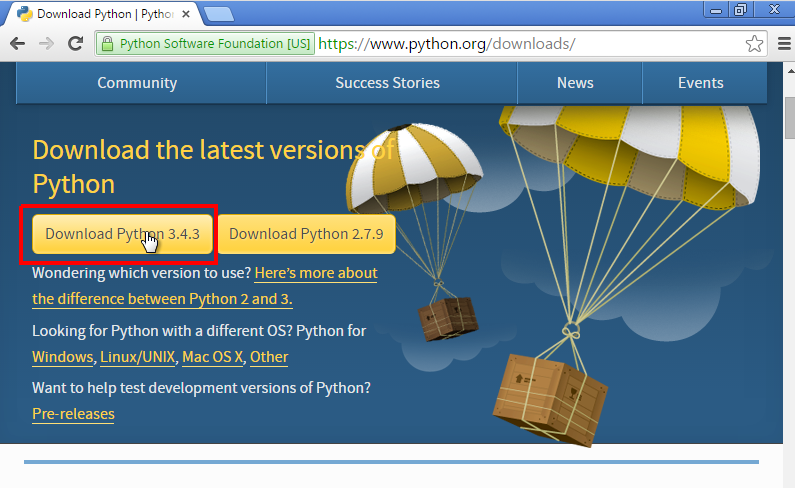
\includegraphics[width=100mm]{bilder/python_download}
\\
\textbf{Hinweis:} Im CoderDojo verwenden wir Python 3, deswegen ist es wichtig den Python 3-Installer herunterzuladen. Die derzeit aktuelle Version ist 3.4.3.
\\
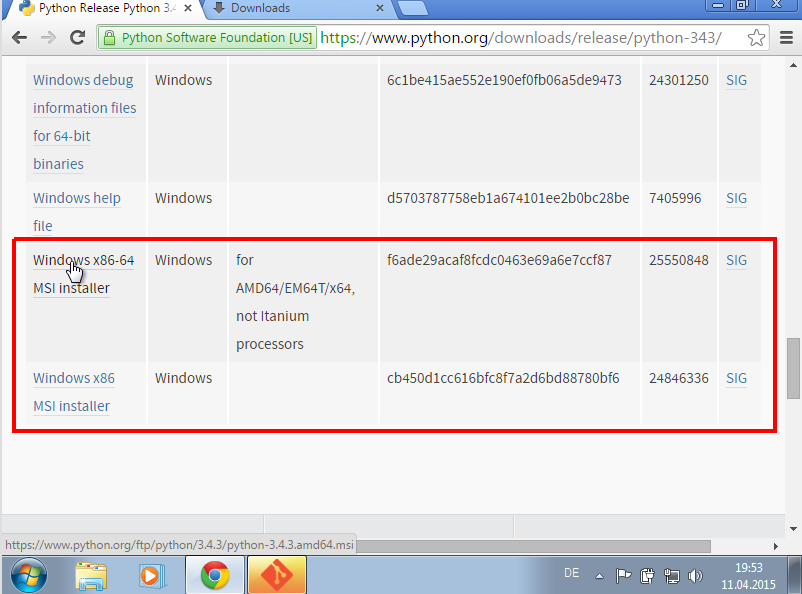
\includegraphics[width=100mm]{bilder/python_download_win}
\\
Falls der Download nicht automatisch startet, muss die korrekte Version von Hand ausgewählt werden. In dem Bild die 64-bit Windows Version, dies ist allerdings abhängig von der installierten Windowsversion.

\clearpage

\subsection{Installation}
Die heruntergeladene Installationsdatei durch Doppelklick starten. In den erscheinenden Fenstern auf "Weiter" und/oder "Ok" klicken um die Installation durchzuführen. Die Voreingestellten Werte (z.B. Installationsverzeichnis) sollten okay sein, können aber natürlich nach belieben geändert werden.
\\
\textbf{Hinweis:} Die Installation erfordert Administratorrechte.
\\


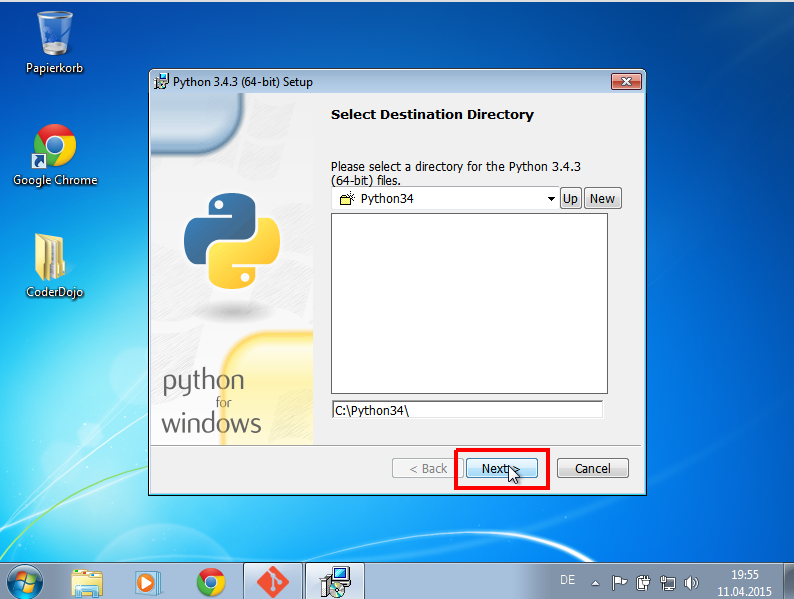
\includegraphics[width=100mm]{bilder/python_install}
\\
Die Installation sollte ohne Probleme durchlaufen. Danach ist Python erfolgreich auf dem System installiert.

\clearpage

\section{Anpassung der Pfad-Umgebungsvariablen}
Um Python einfacher auf der Rechner nutzen zu können ist es empfehlenswert den Installationsordner zur Pfad-Umgebungsvariblen hinzuzufügen. Programme derren Installationsordner in der Pfad-Umgebungsvariablen stehen können direkt über ihren Namen aufgerufen werden.
\\
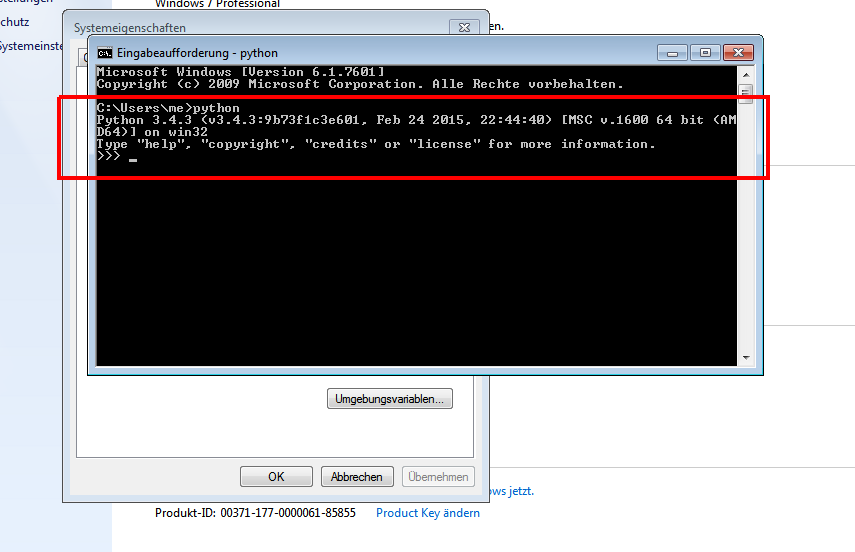
\includegraphics[width=100mm]{bilder/cmd_python}
\\
Python kann dann direkt von der Kommandozeile/Konsole verwendet werden.

\subsection{Finden der Umgebungsvariablen}
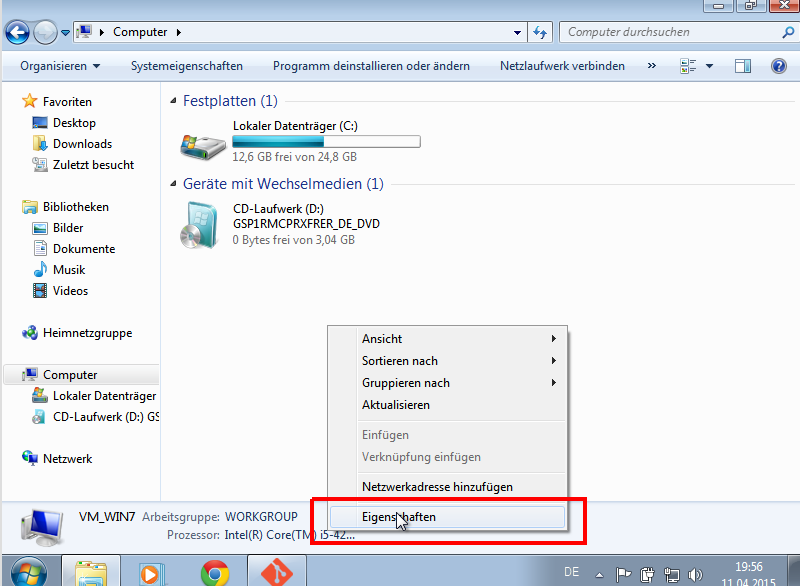
\includegraphics[width=100mm]{bilder/computer_properties}
\\
Diese sind mittels Rechtsklick auf "Computer/Arbeitsplatz" -\textgreater "Eigenschaften" ...
\\
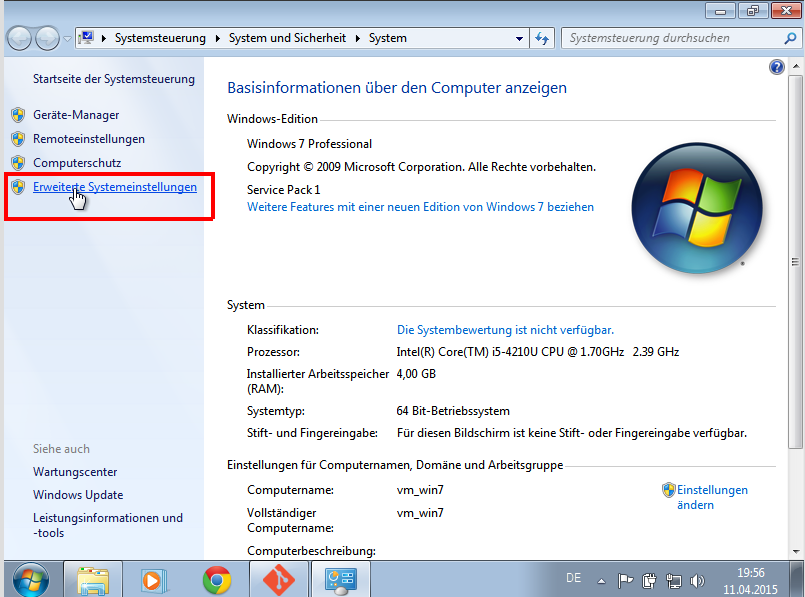
\includegraphics[width=100mm]{bilder/advanced_properties}
\\
... unter "Erweiterte Systemeinstellungen" ...
\\
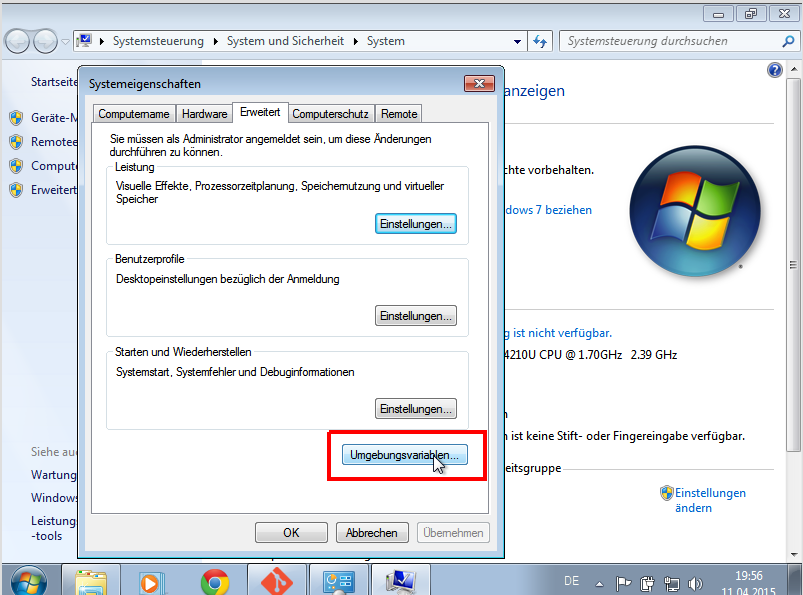
\includegraphics[width=100mm]{bilder/sys_vars}
\\
... zu finden.

\clearpage
\subsection{Anpassen der Pfad-Umgebungsvariablen}
Nun muss aus der Liste der Umgebungsvariablen die "Pfad"/"Path" ausgewählt werden.
Durch Klicken auf "Bearbeiten..." öffnet sich ein Dialog zum Bearbeiten der Pfad-Umgebungsvariablen.
\\
\textbf{Hinweis:} Das Ändern der Pfad-Umgebungsvariablen erfordert Administratorrechte.
\\
Außerdem ist Vorsicht geboten beim Bearbeiten der Pfad-Variablen. Sollte diese aus Versehen gelöscht oder fehlerhaft bearbeitet werden, kann dies Auswirkungen auf andere Programme haben kann!
\\
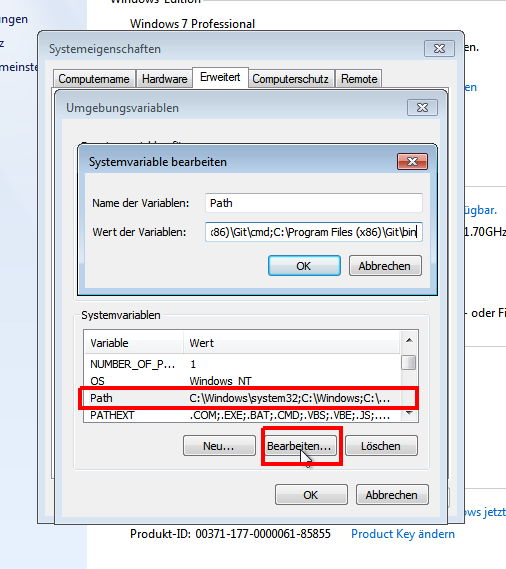
\includegraphics[width=100mm]{bilder/edit_path}
\\
Die Pfad-Umgebungsvariable ist eine Liste von Verzeichnispfaden, die mit ';' getrennt geschrieben sind.
\\
Nun muss am Ende mit ';' das Python-Installationsverzeichnis einfgefügt werden. Das Standartverzeichnis für Python 3.4 ist "C:\textbackslash Python34 \textbackslash". Der Pfad muss allerdings gegebenenfalls angepasst werden!
\\
Optional kann auch das "Scripts"-Verzeichnis im Python-Ordner zur Pfad-Variablen hinzugefügt werden. Dies hilft, falls später später bspw. mittesls "pip" weitere Python-Module installiert werden sollen.
\\
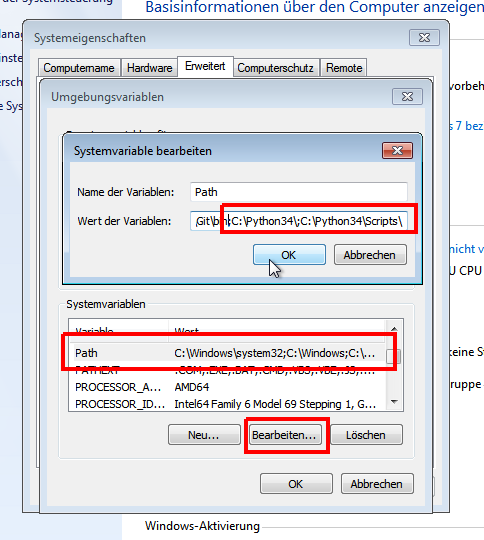
\includegraphics[width=100mm]{bilder/python_path}
\\
Nach Bestätigung über "Ok" und Schleißen der Fenster sollte die Pfadvariablen korrekt gesetzt sein. Dies kann überprüft werden indem man die Windowskommandozeile  öffnet und "python" eintippt und mit der Enter-Taste bestätigt. Die Kommandozeile kann man durch Suchen von "cmd" im Windows-Suchfeld finden.
\\
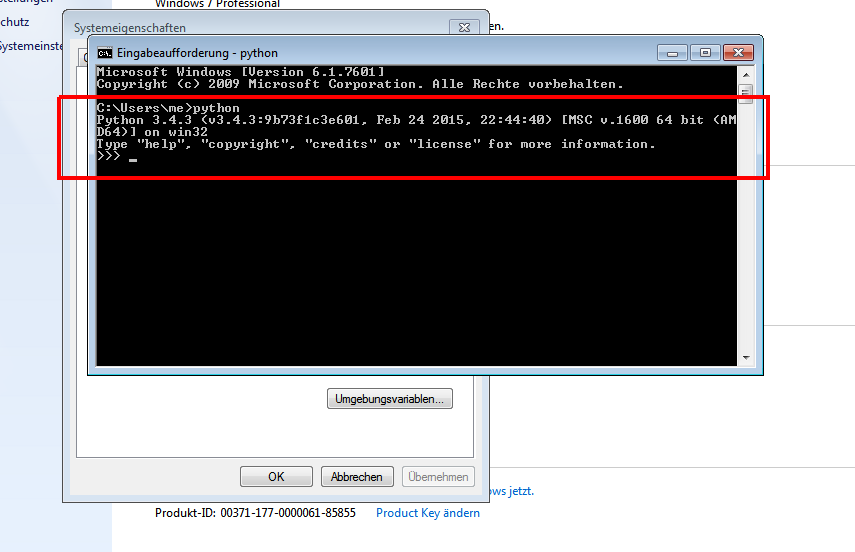
\includegraphics[width=100mm]{bilder/cmd_python}
\clearpage

\section{Editor}
Die Installation von Python sollte jetzt komplett sein. Nun ist nur noch die Frage zu klären, wie und mit welchem Programm Python programmiert werden kann.
\\
\subsection{IDLE}
Standartmäßig kommt mit Python die IDLE (Integrated Development Environment), die benutzt werden kann. Diese ist allerdings nicht allzu komfortabel zu benutzen, besitzt allerdings alle Wesentlichen Funktionen. Die englische Dokumentation ist hier: \url{https://docs.python.org/3.4/library/idle.html} zu finden.
\\
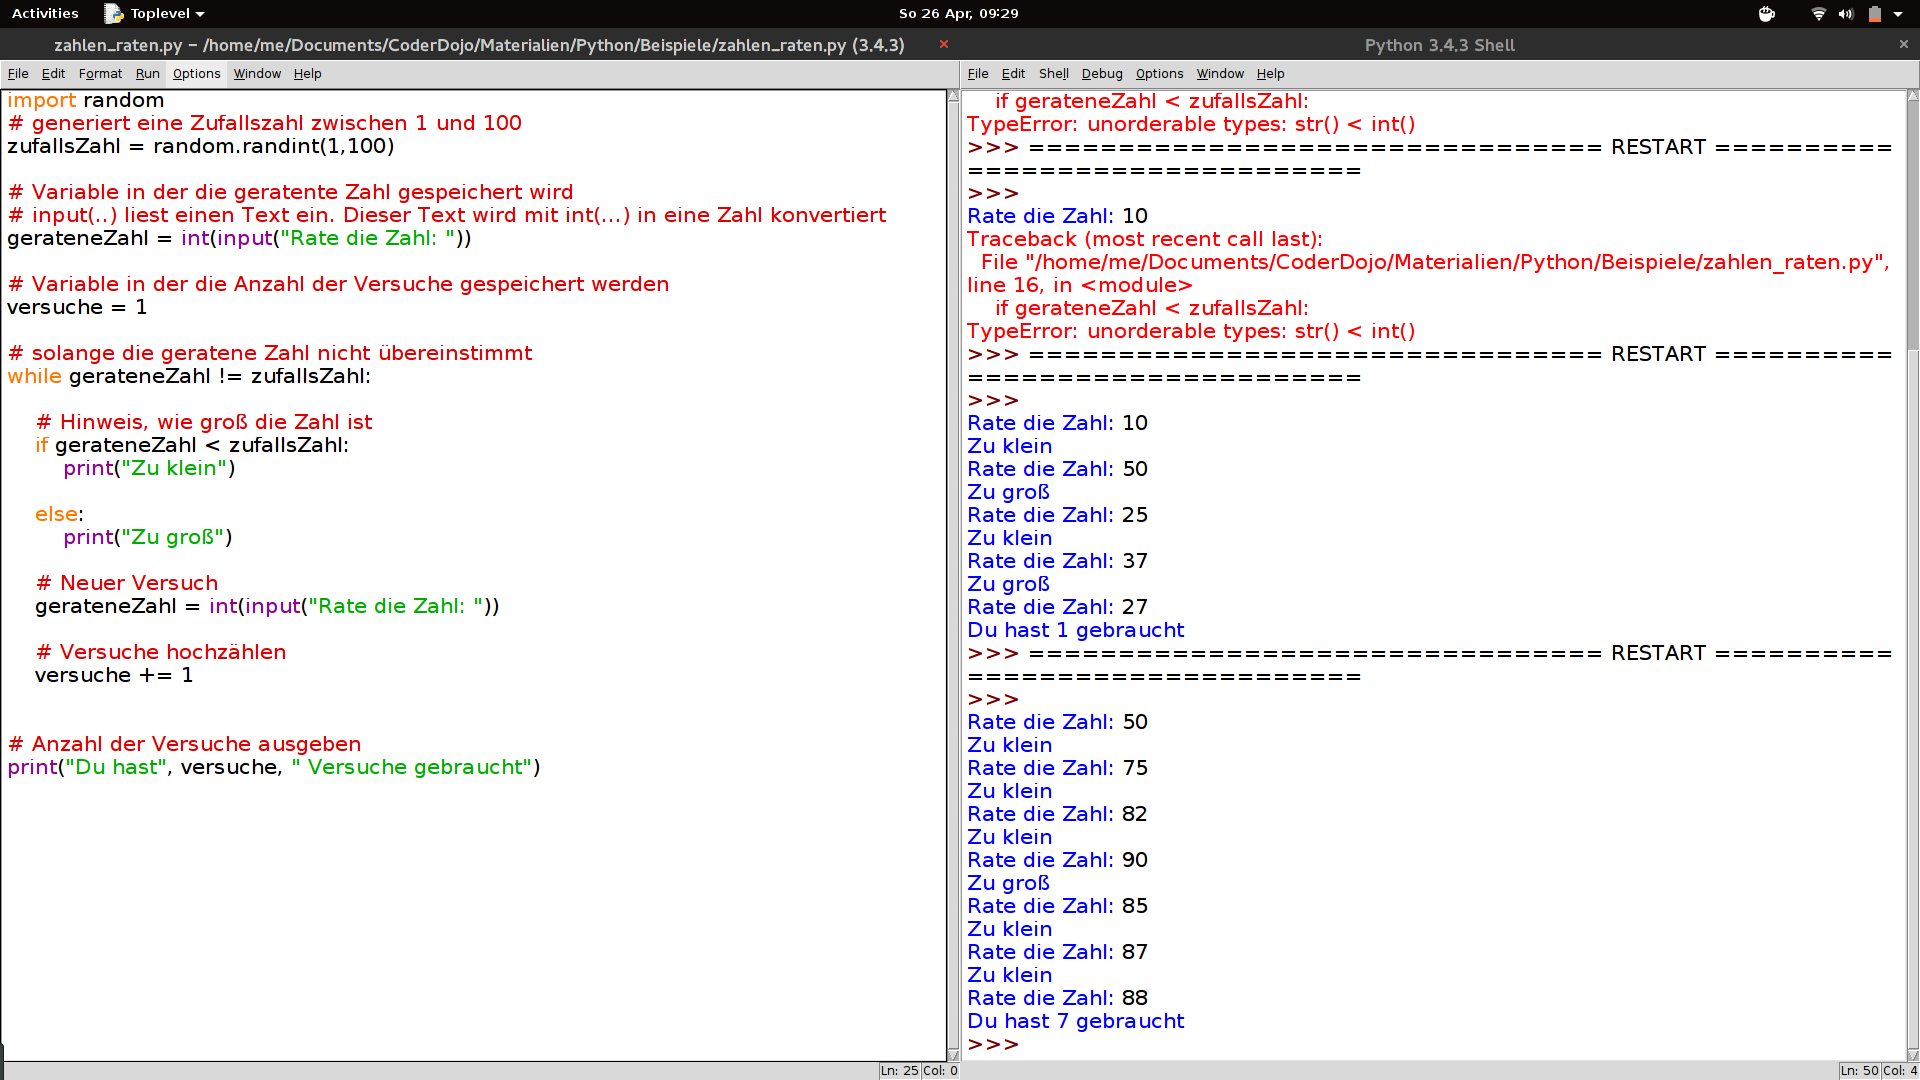
\includegraphics[width=150mm]{bilder/idle}
Unter "File -\textgreater New" kann einen neue Datei erstellt werden. Unter "Run -\textgreater Run Module (F5)" kann die Datei ausgeführt werden. Dies öffnet ein "Python Shell Fenster". Es empfiehlt, solange der Bildschirm groß genug ist, beide Fenster nebeneinander zu haben.
\\


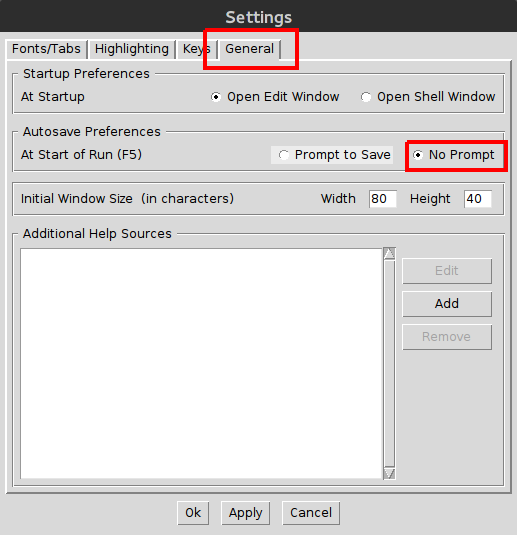
\includegraphics[width=100mm]{bilder/auto_save}
\\
Um die Datei auszuführen, ist es gut sich die Tastenkombination "F5" zum Ausführen zu merken und zu benutzen. Dafür ist es außerdem hilfreich, wenn man in den Einstellungen unter "Options -\textgreater Configure IDLE" im "General"-Tab die Einstellung bei "Autosave Preferences" auf "No Prompt" setzt, damit die Datei automatisch beim Ausführen gespeichert wird.

\end{document}
